%% ============================================================
%%  SECCIÓN 10 — Gráficas
%% ============================================================

\section{Gráficas}
\label{sec:graficas}

En esta sección se presentan las representaciones gráficas de los resultados experimentales generadas mediante el script computacional~\cite{script_graficas} empleando las librerías científicas \texttt{NumPy}~\cite{numpy}, \texttt{Matplotlib}~\cite{matplotlib} y \texttt{SciPy}~\cite{scipy}.

\begin{figure}[H]
    \centering
    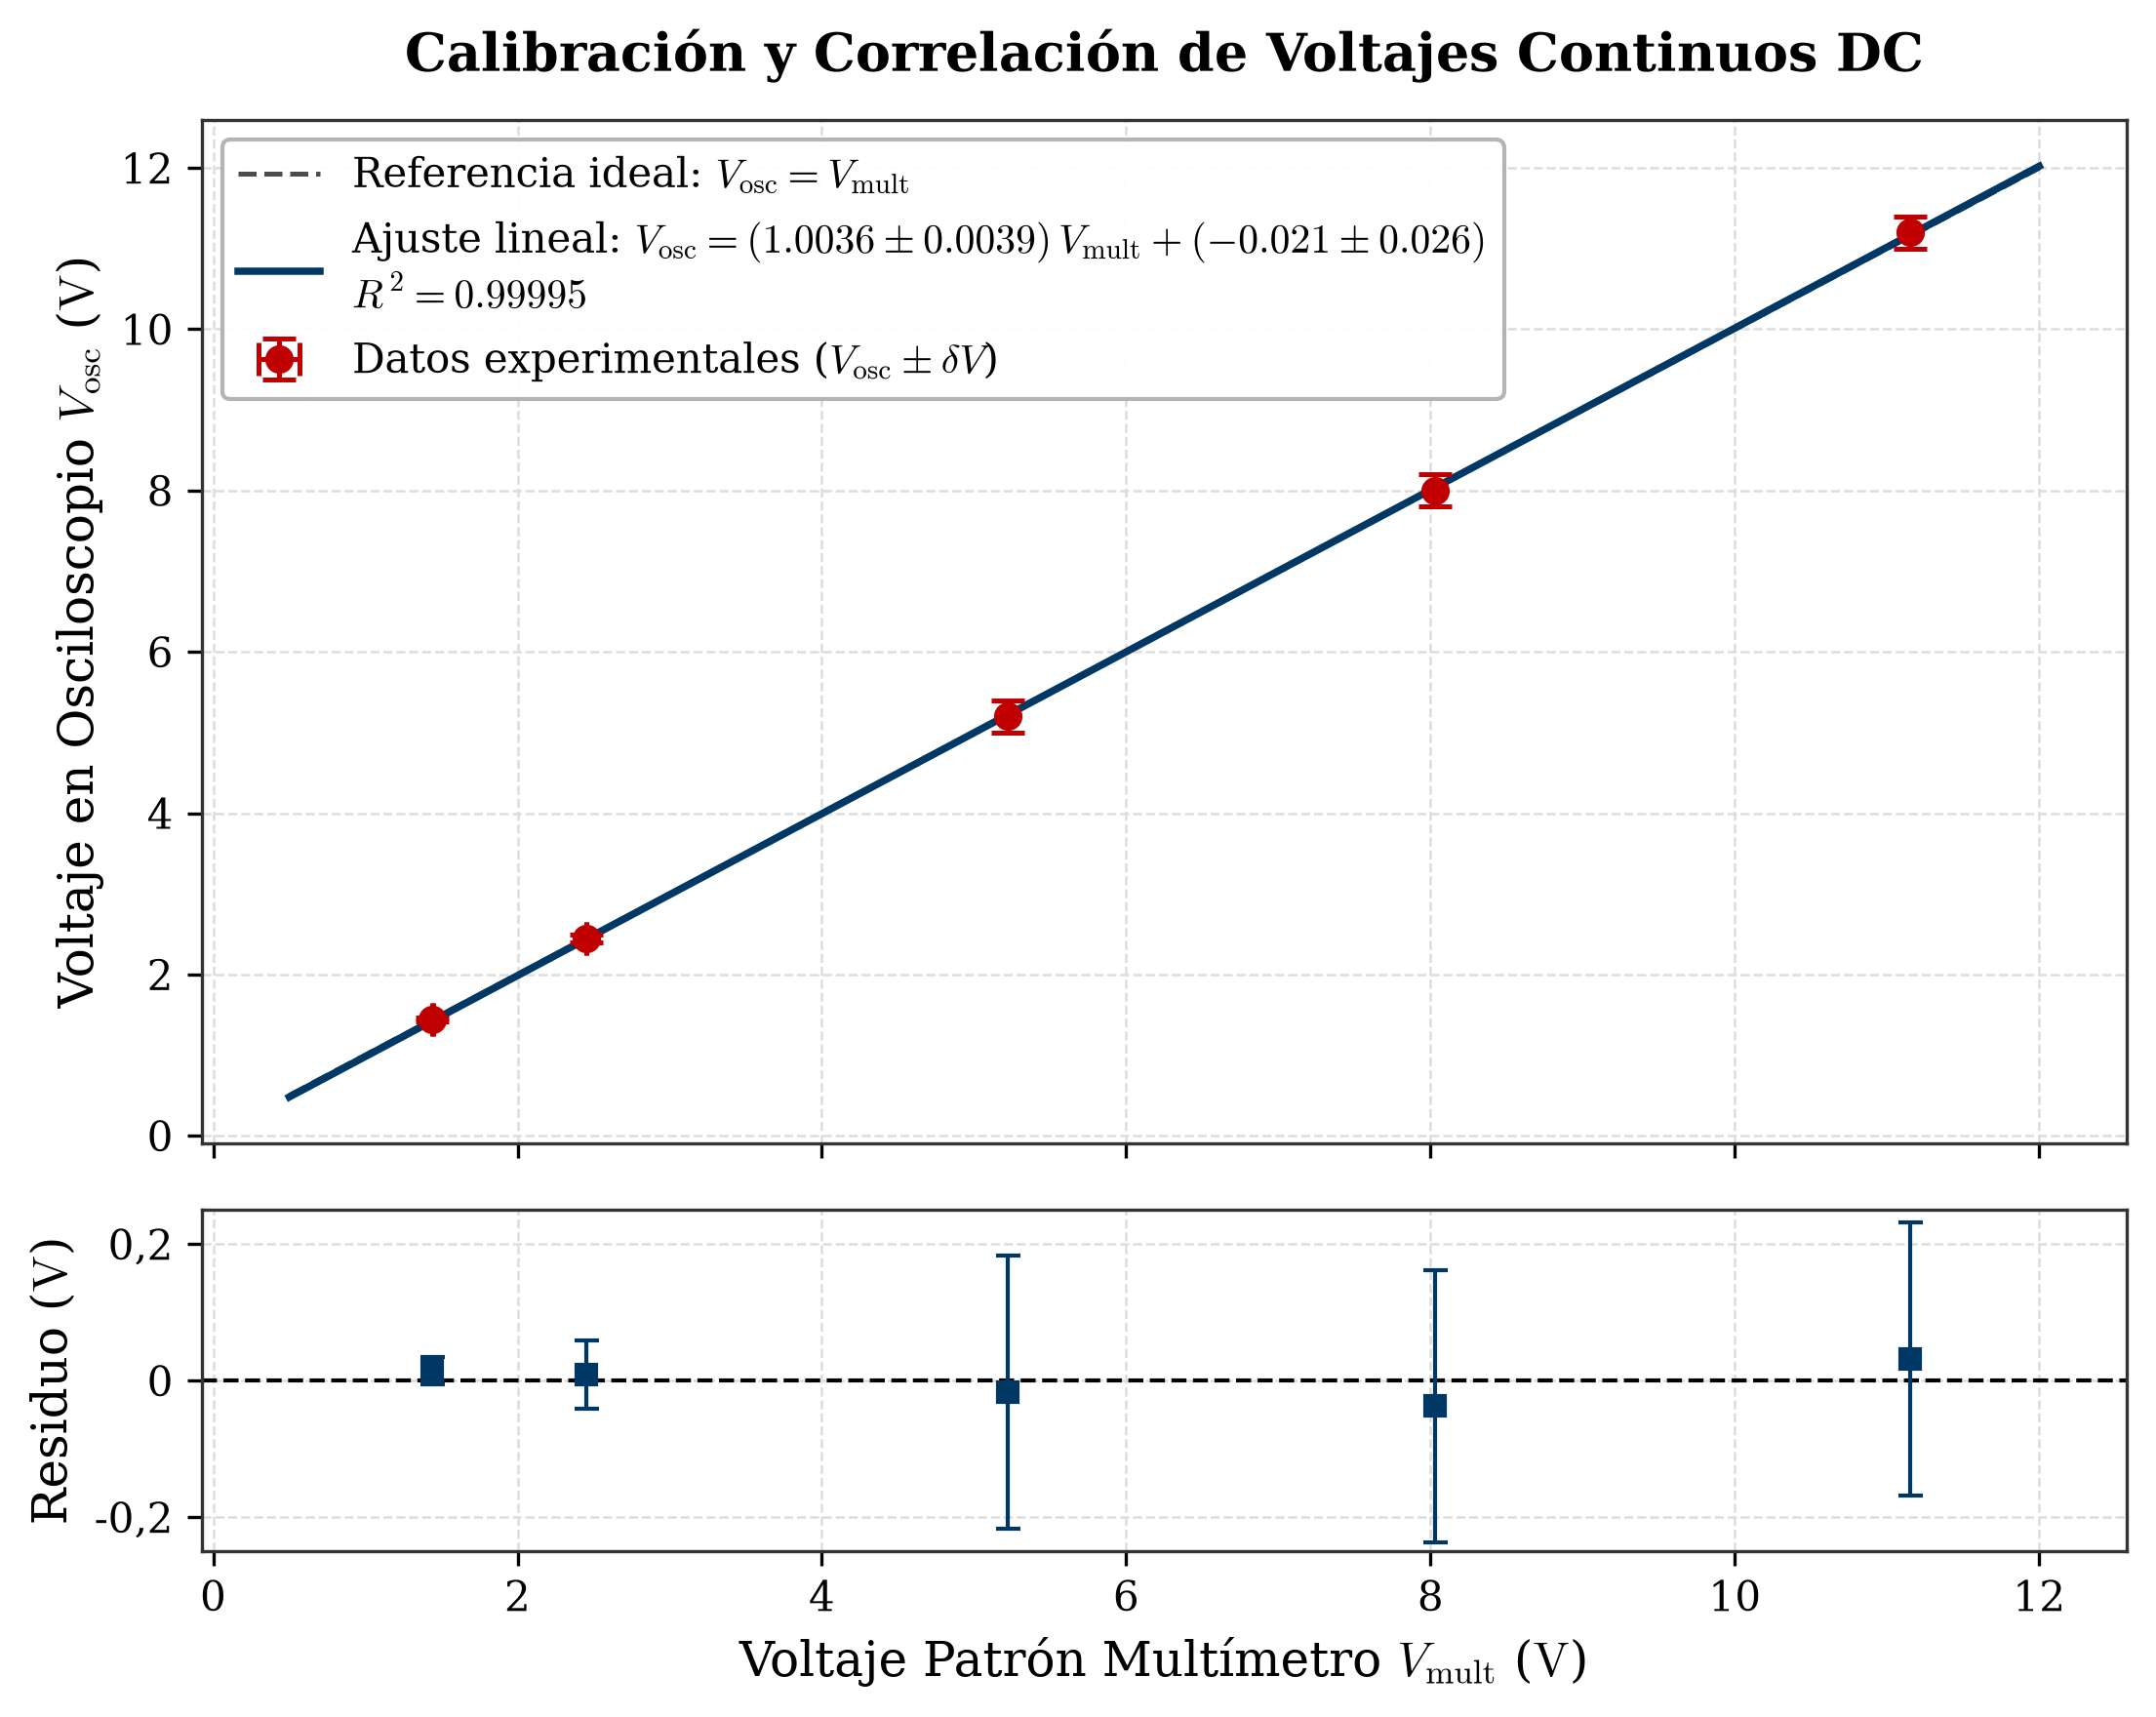
\includegraphics[width=0.85\linewidth]{grafica_calibracion_dc}
    \caption{Curva de calibración y correlación de voltajes continuos (DC). El panel superior muestra los datos experimentales ($V_{\text{osc}} \pm \delta V$) en escala óptima frente al multímetro patrón ($V_{\text{mult}}$), la recta ideal $y = x$ y el ajuste por mínimos cuadrados ($R^2 = 0{,}99995$). El panel inferior detalla los residuos de ajuste con sus barras de error instrumental. Generado con \texttt{Matplotlib}~\cite{matplotlib} y \texttt{SciPy}~\cite{scipy} según el script~\cite{script_graficas}.}
    \label{fig:calibracion_dc}
\end{figure}

\begin{figure}[H]
    \centering
    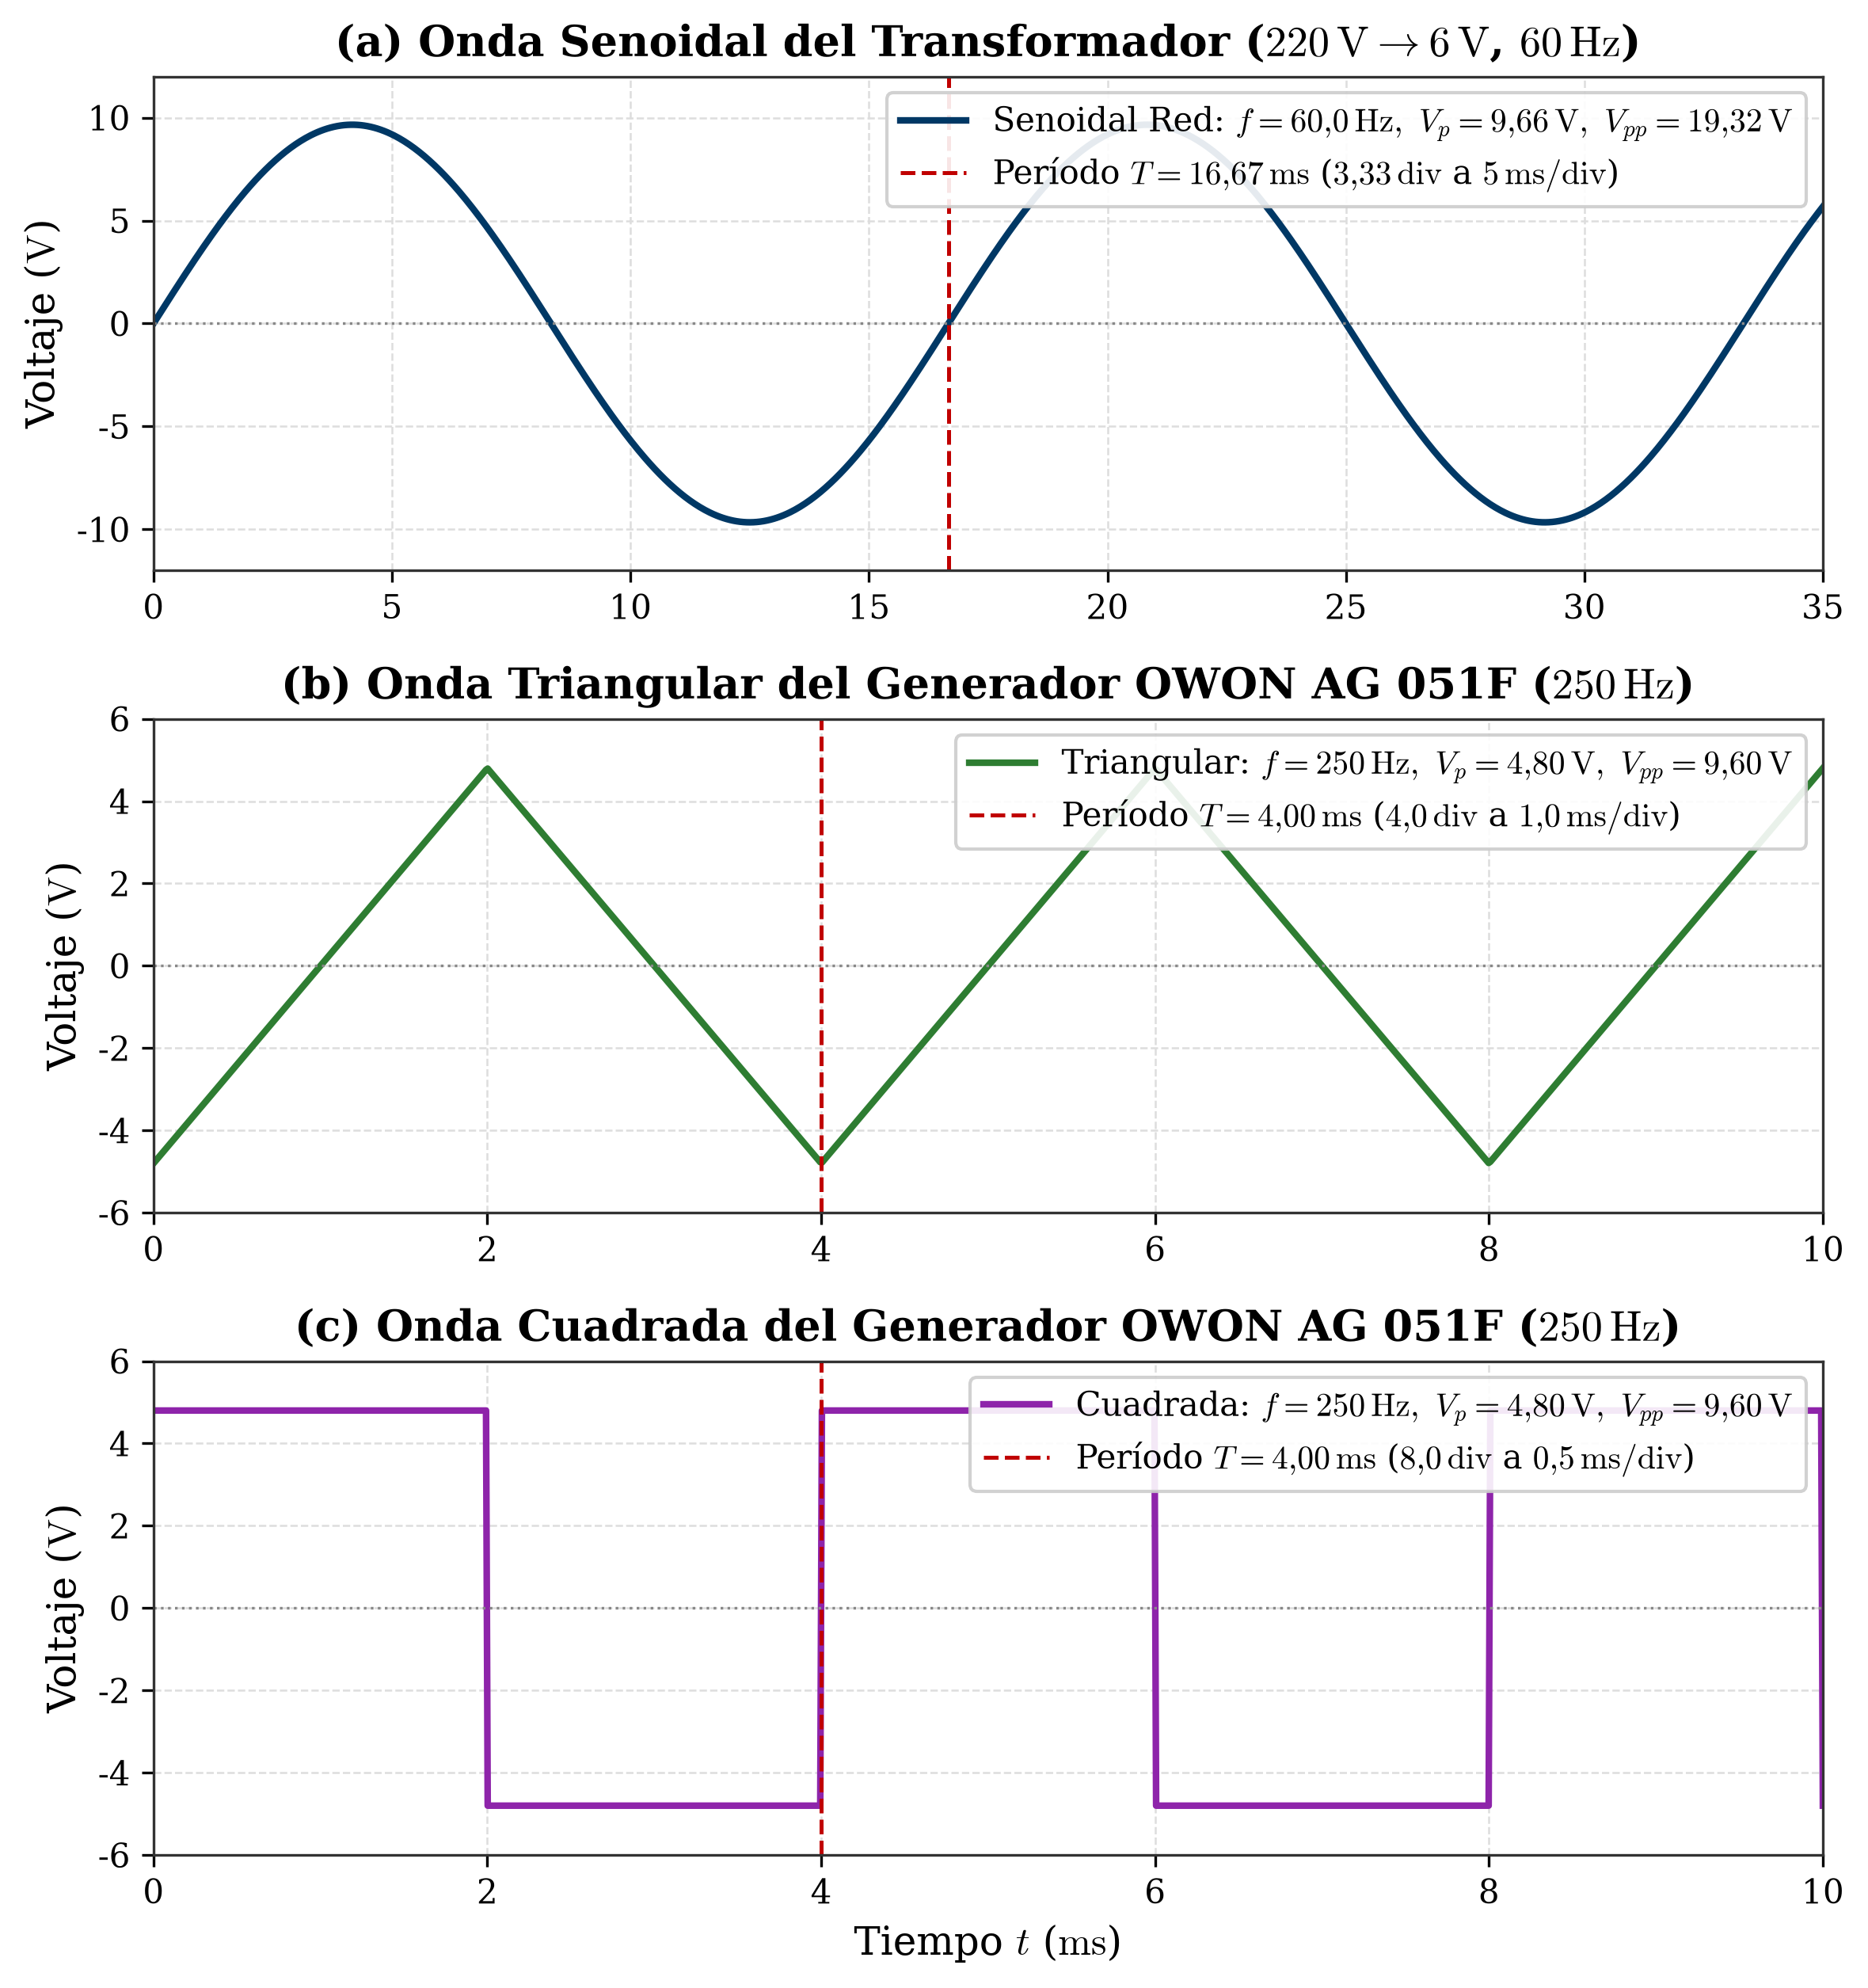
\includegraphics[width=0.88\linewidth]{grafica_ondas_ac}
    \caption{Representación en el dominio del tiempo de las formas de onda alternas registradas: (a) Tensión senoidal del transformador reductor ($f = \qty{60,0}{\hertz}$, $V_p = \qty{9,66}{\volt}$, $V_{pp} = \qty{19,32}{\volt}$, $T = \qty{16,67}{\milli\second}$); (b) Onda triangular del generador OWON AG 051F ($f = \qty{250}{\hertz}$, $V_p = \qty{4,80}{\volt}$, $T = \qty{4,00}{\milli\second}$); (c) Onda cuadrada del generador OWON AG 051F ($f = \qty{250}{\hertz}$, $V_p = \qty{4,80}{\volt}$, $T = \qty{4,00}{\milli\second}$). Procesado mediante~\cite{numpy, matplotlib, script_graficas}.}
    \label{fig:ondas_ac}
\end{figure}

\begin{figure}[H]
    \centering
    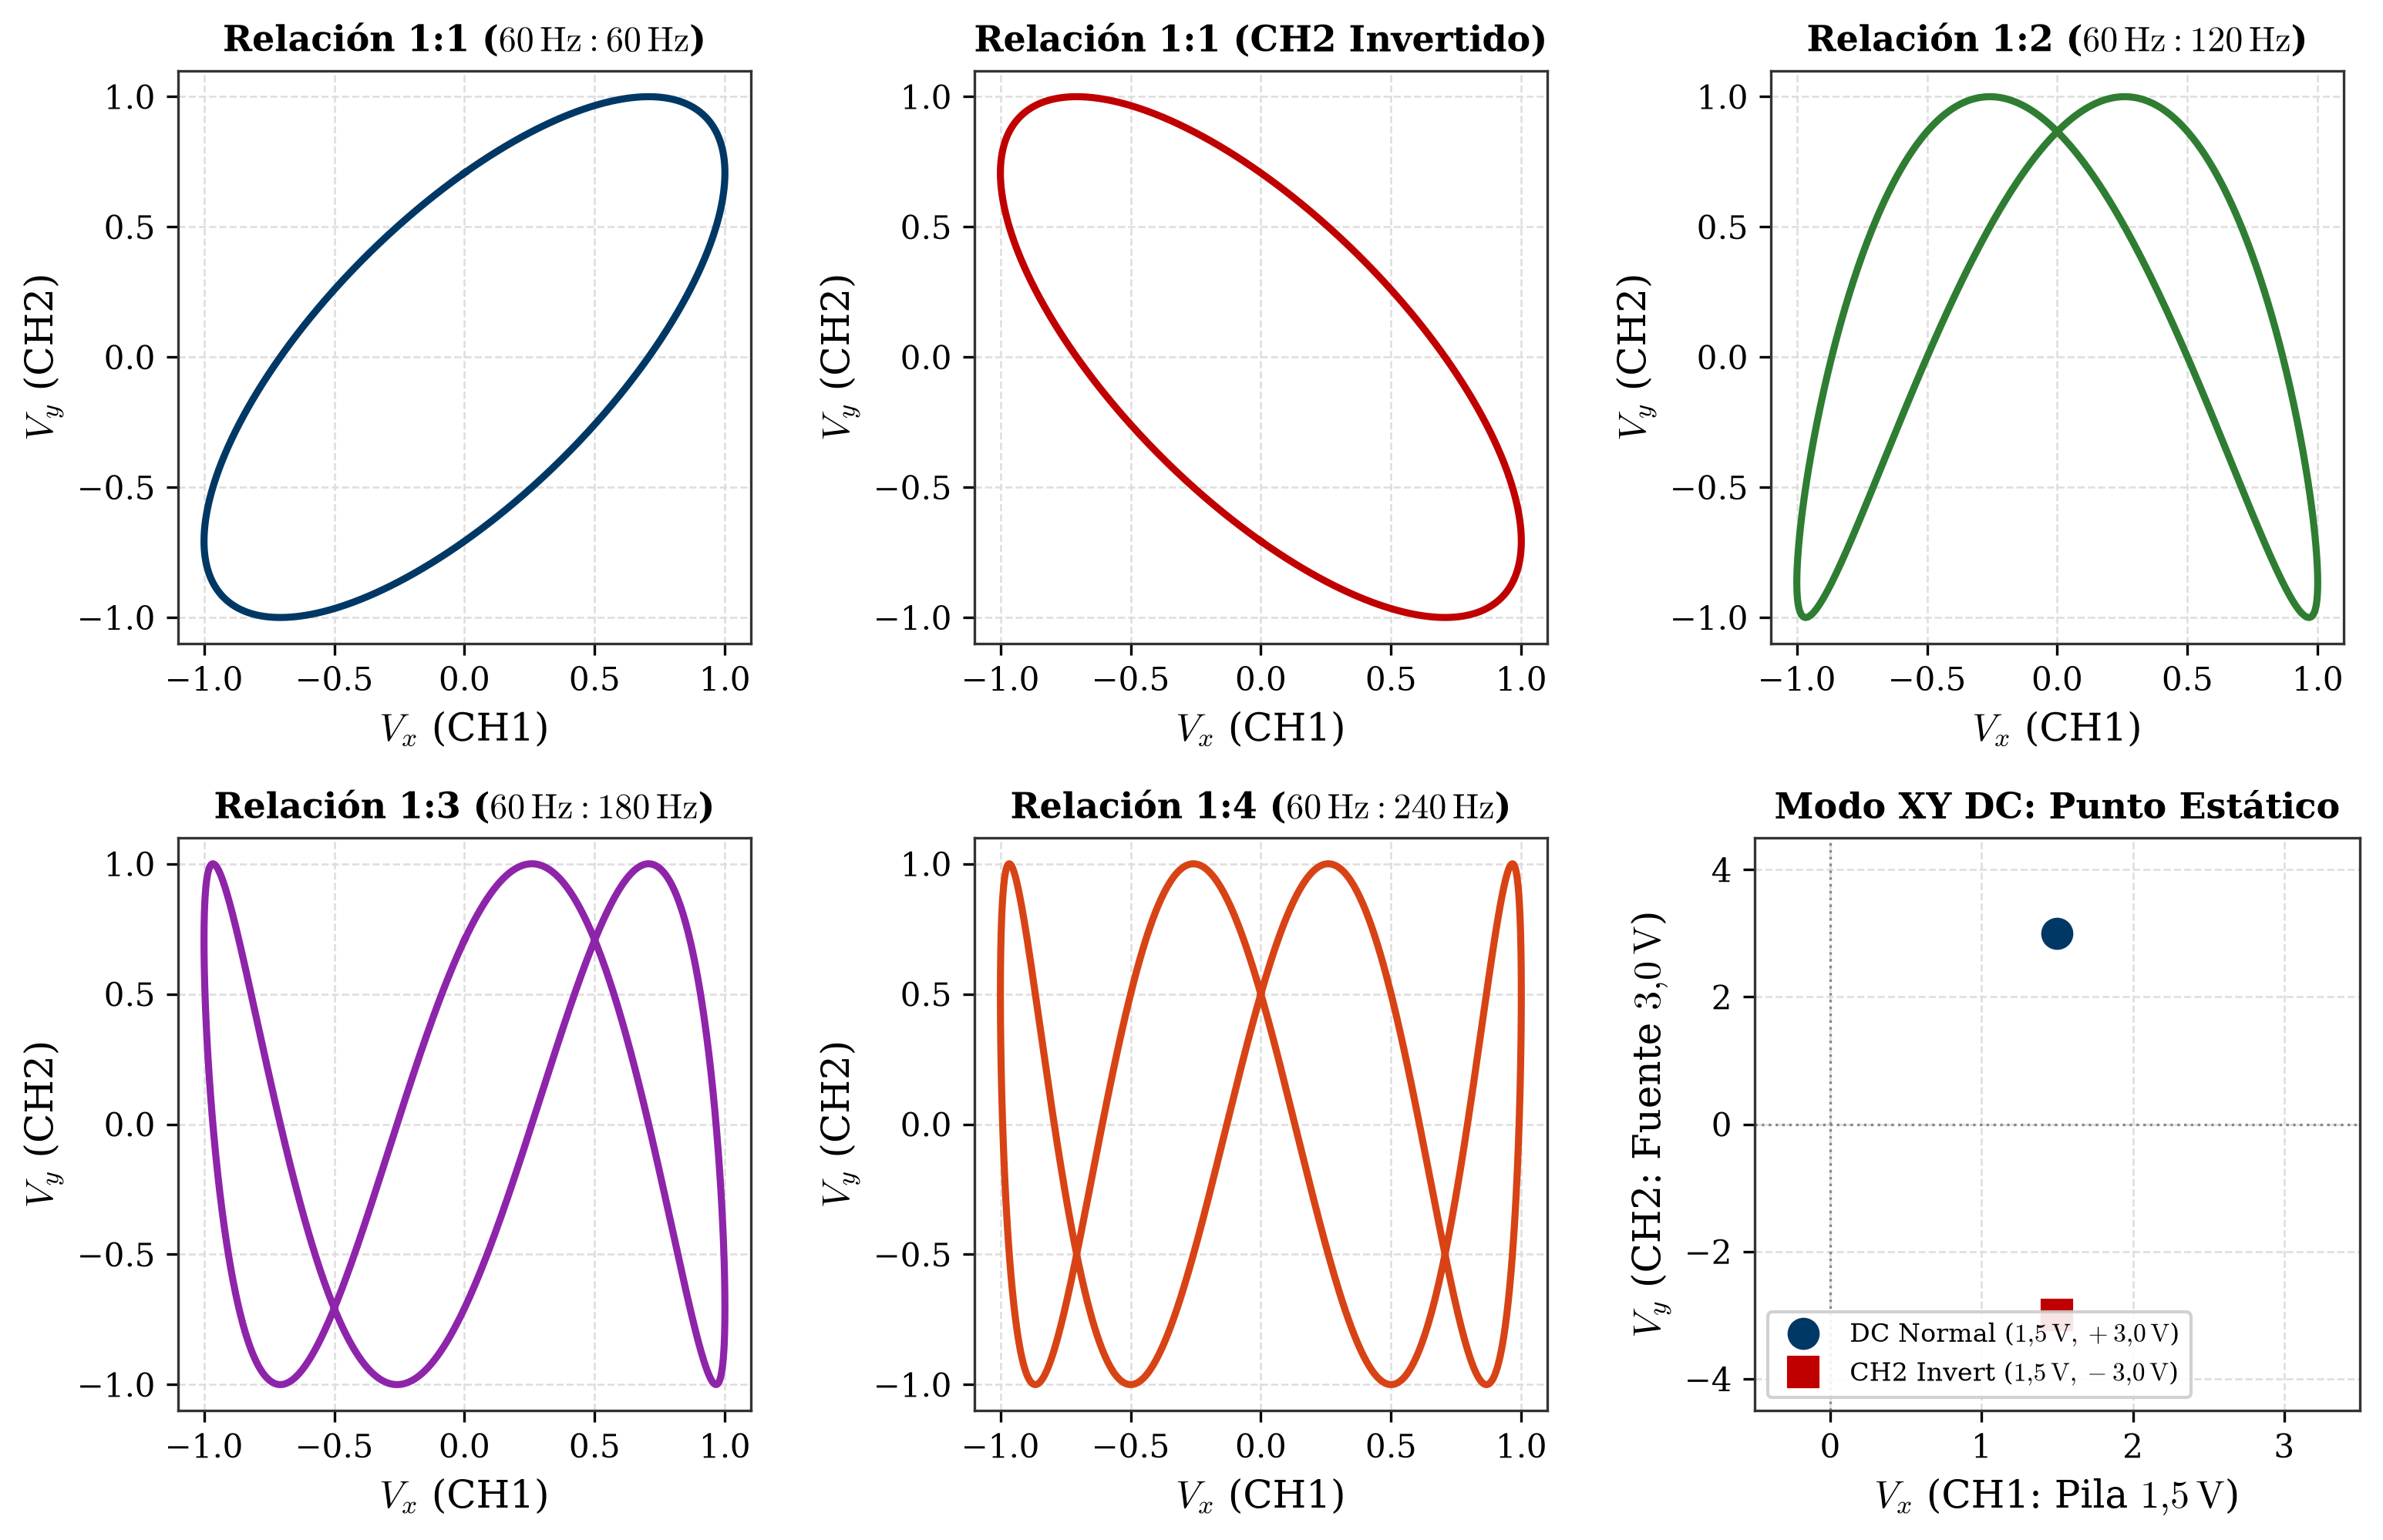
\includegraphics[width=0.95\linewidth]{grafica_lissajous_xy}
    \caption{Trayectorias en el modo graficador bidimensional $X$-$Y$ y figuras de Lissajous: Relaciones armónicas $1:1$ normal y con canal $\text{CH2}$ invertido ($y \to -y$), relaciones enteras $1:2$ (\qty{120}{\hertz}), $1:3$ (\qty{180}{\hertz}) y $1:4$ (\qty{240}{\hertz}), y proyección de puntos estáticos para señales continuas DC (\qty{1,5}{\volt}, $\pm\qty{3,0}{\volt}$). Generado según el script~\cite{script_graficas}.}
    \label{fig:lissajous_xy}
\end{figure}
